\documentclass[11pt]{article}
\usepackage[utf8]{inputenc}
\usepackage[T2A]{fontenc}
\usepackage{graphicx}
\begin{document}
\title{Отчёт: таблица и рисунок}
\author{python\_hws}
\maketitle

\begin{tabular}{|c|c|c|}
\hline
Тема & Баллы & Статус \\
\hline
Таблицы в LaTeX & 10 & Сдано \\
\hline
Рисунки в LaTeX & 10 & Сдано \\
\hline
Итого & 20 & --- \\
\hline
\end{tabular}

\begin{figure}[htbp]
\centering
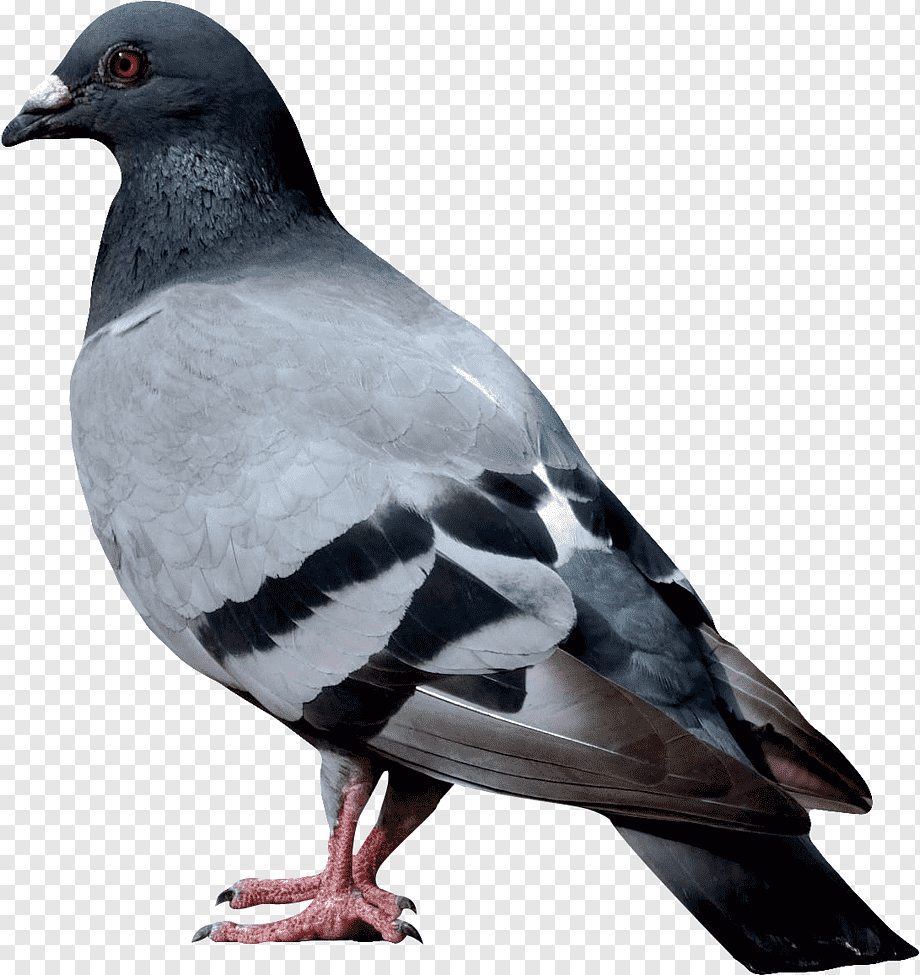
\includegraphics[width=0.35\textwidth]{image.png}
\caption{Пример рисунка}
\end{figure}
\end{document}